\documentclass[letterpaper, 11 pt]{article}
\usepackage{siunitx}
\usepackage{natbib}

%Image pkgs
\usepackage{float}
\usepackage{graphicx}
\graphicspath{ {images/} }
\usepackage{subcaption}

%Algorithm display pkgs
\usepackage{algorithm} 
\usepackage{algpseudocode}

%Math pkgs
\usepackage{amsmath}
\usepackage{breqn}

%Content formatting
\addtolength{\oddsidemargin}{-.875in}
\addtolength{\evensidemargin}{-.875in}
\addtolength{\textwidth}{1.75in}

\addtolength{\topmargin}{-.875in}
\addtolength{\textheight}{1.75in}

\title{\Large \bf Auger-driven Motion in Granular Media}
\author{\centering Stephanie L. Chang and Paul B. Umbanhowar}

\begin{document}
\pagenumbering{arabic}
\maketitle

\begin{abstract}
The purpose of this project was to create an underground locomotor capable of following user-defined, arbitrary trajectories. Using FDM 3D printing, numerous iterations of a modular robot mounted with an auger were fabricated. Rapid, empirical tests within a loosely packed bed of poppy seeds were performed to clarify how certain auger parameters influenced the behavior of the robot in the horizontal plane. A theoretical model was derived to describe how the parameters of an auger and granular material characteristics can affect the amount of propulsive force generated.   

\end{abstract}

\tableofcontents

\section{Introduction}

Why this project is interesting and important for the industry today
Goal underground locomotor follow arbitrary trajectories
Many geometries tried Maladen, push me pull me, etc. 

Description on how I intended to build and test a robot in poppy seeds and created a mathematical model based off of Francisco's recent paper to optimize the parameters.  
Wings to counteract torque.

Initial idea to make and try.

Describe why we built it as it was and why we decided not to go with certain designs like the double screw. Modular for easy assembly and localized testing. 

\section{Iteration Progression}

The robot consists of 5 main components. When powered, an Archimedes screw mounted at the head of the robot will spin to part granular media and pull the robot forward. This is attached to an adapter plate which fits snugly around the shaft of a DC motor. A cylindrical cap on the motor itself stops granules from falling into an exposed gear box. Wedged inside the protective cap are wings which prevent the body of the robot from rotating with the screw. Lastly, an elongated hemispherical housing unit covers the back of the robot to shield soldered wire junctions from wear and tear. Note, a modular robot was created to make testing different combinations of screws and wing shapes easier.

\begin{figure}[H]
\centering
\includegraphics[width=0.7\linewidth]{./imgs/augerbot}
\caption{The first prototype of the augerbot}
\label{fig:augerbot}
\end{figure}

\begin{figure}[H]
\centering
\includegraphics[width=0.7\linewidth]{./imgs/all_screws}
\caption{All augers tested}
\label{fig:all_screws}
\end{figure}

Describe what was seen with the first blind test. Problems encountered. 
How the following iterations were changed to compensate. 
Wider screw, modular wings, captured nuts for easier assembly and better interfacing with adapter, brass adapter for motor shaft to counter wt imbalance and keep the screw on since the PLA kept wearing after a while.

\section{Analytical Optimization}
During testing, screws with larger radii and pitches appeared to produce more propulsive force. To find the optimal parameters needed to maximize an auger's pulling ability, a more principled method - inspired by extant studies - was developed \cite{Melo,Chen}.

\begin{figure}[H]
\centering
\begin{subfigure}{.5\textwidth}
	\centering
	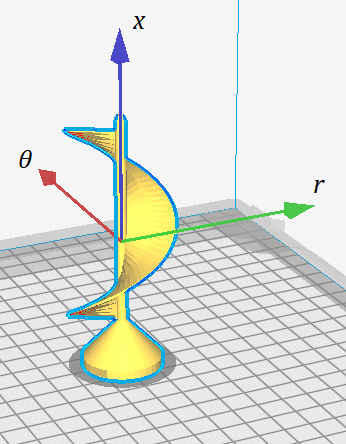
\includegraphics[height=7.5cm]{./imgs/helix_csys}
	\caption{The body coordinate system}
	\label{fig:helix_csys}
\end{subfigure}%
\begin{subfigure}{.5\textwidth}
	\centering
	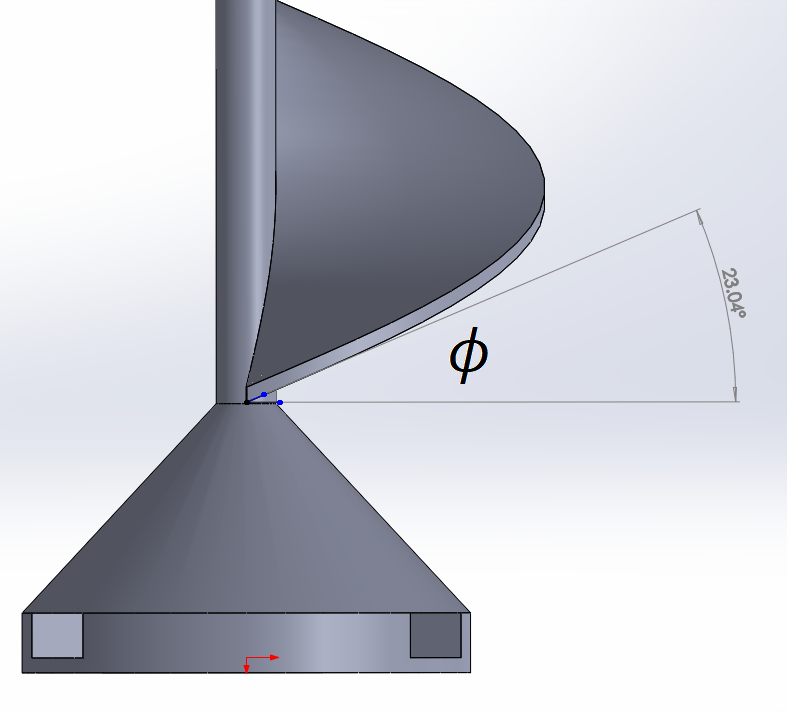
\includegraphics[height=6cm]{./imgs/helix_phi}
	\caption{Local inclination angle $\phi$ is an implicit parameter that depends on the pitch of the helix. It quantifies how far an auger tilts up at an arbitrary point along its perimeter.}
	\label{fig:helix_phi}
\end{subfigure}
\caption{General problem set-up shown on an auger}
\label{probSetup}
\end{figure}
 
A cylindrical coordinate system ($\vec{e_r}, \vec{e_\theta}, \vec{e_x}$) was used to describe the helix [Figure~\ref{fig:helix_csys}]. Local inclination angle $\phi$, shown in Figure~\ref{fig:helix_phi}, was used to define tangential unit vector $\vec{e_t} = \left\langle 0, \cos(\phi),\sin(\phi)\right\rangle $ and normal unit vector $\vec{e_n} = \left\langle 0, \sin(\phi), -\cos(\phi)\right\rangle $. For a tiny segment along the helix path, the local velocity was determined to be $\vec{\nu} = \left\langle 0, rw, U\right\rangle $, where $\omega$ represents the angular velocity about the auger's stem and $U$ refers to the translational velocity along the x-axis. Note, the screw's radius and height were restricted to account for the dimensions of the poppy seed tank and the build volume of the Ultimaker 3 3D printer.  

Imagine an auger is composed of infinitesimal segments, each of which feels drag and thrust. According to resistive force theory (RFT), the amount of force generated by a body moving through granular media can be approximated by adding the forces experienced by each of its finite elements. $F_x(\phi,U)$, therefore, is the linear superposition of all local forces projected onto the x-axis. For an auger with radius $R$ and $n$ revolutions, this calculation looks like
\begin{equation}\label{FxBasic}
F_x(\phi,U) = \int_{0}^{R}\int_{0}^{2\pi n} (\vec{f}\cdot\vec{e_x})\frac{r}{\cos(\phi)} d\theta dr\ \text{,}
\end{equation}
where $\vec{f}$ denotes the force per unit area felt by each partition. Coulomb's law of friction was used to express $\vec{f}$ as the sum of two force components tangential and normal to stem of the auger. Fleshed out, this equation takes the form
\begin{equation}\label{f}
\begin{split} 
\vec{f} &= -C_t(\vec{e_\nu}\cdot\vec{e_t})\vec{e_t}-C_n(\vec{e_\nu}\cdot\vec
{e_n})\vec{e_n} \\
&=\frac{-C_t(r\omega\cos(\phi)+U\sin(\phi))\vec{e_t}-C_n(r\omega\sin(\phi)-U\cos(\phi))\vec{e_n}}{\sqrt{U^2+(r\omega)^2}}\ \text{,}
\end{split} 
\end{equation}
where $C_t$ and $C_n$ represent depth- and $\phi$- dependent tangential and normal stress coefficients respectively. 

Plugging equation (\ref{f}) into equation (\ref{FxBasic}), the total amount of propulsive force generated by the auger in the x-direction was found to be  
\begin{dmath}\label{FxAuger}
F_x(\phi,U) = \frac{2\pi n}{\cos(\phi)}\left[(C_n-C_t)\omega\sin(\phi)\cos(\phi)\left( \frac{R}{2\omega^2}\sqrt{(R\omega)^2+U^2}+\frac{U^2}{2\omega^3}\left( \ln\frac{U}{R\omega+\sqrt{(R\omega)^2+U^2}}\right) \right) \\
- \frac{U}{\omega^2}(C_t\sin^2(\phi)+C_n\cos^2(\phi)(\sqrt{(R\omega)^2+U^2}-U) \right] 
\end{dmath}
where $\vec{e_x} = \left\langle 0,0,1 \right\rangle $. Introducing non-dimensional helix velocity $\tilde{U} = \frac{U}{R\omega}$, equation (\ref{FxAuger}) was rearranged as follows
\begin{dmath}\label{NDFxAuger}
F_x(\phi, \tilde{U}) = \frac{2\pi R^2n}{\cos(\phi)}\left[\frac{1}{2}(C_n-C_t)\sin(\phi)\cos(\phi)\left[\sqrt{1+\tilde{U}^2}+\tilde{U}^2\ln\left(\frac{\tilde{U}}{1+\sqrt{1+\tilde{U}^2}} \right)  \right] \\
- \tilde{U}(C_t\sin^2(\phi)+C_n\cos^2(\phi))\left(\sqrt{1+\tilde{U}^2}-\tilde{U}\right) \right]\ \text{.} 
\end{dmath}
When the system is at equilibrium, $\phi$ is the only parameter that controls the value of $U$. Recall, $C_t$ and $C_n$ both depend on $\phi$. The steady-state case is important because, when thrust and drag are balanced, $U$ is the constant velocity at which the auger advances along the x-direction. Algorithm 1, therefore, systematically varies $\phi\in\left(0,\frac{\pi}{2} \right] $ to find the $\phi_{opt}$ value which yields the highest $U$.  

\begin{algorithm}[H]
	\caption{Helix Local Inclination Optimization}
	\label{augerOpt}
	
	\begin{algorithmic} %Program set-up
	\State \textbf{Knowns:}
	\State $R, n, d, \omega$ \Comment Auger radius, number of turns, auger depth, and angular velocity
	\State $0<\varepsilon \ll 1$
	\State $F_x(\phi,U)$ \Comment Propulsive force generated in the horizontal direction
	\State
	\State \textbf{Compute:} Maximum helix translational velocity $U$ for different $\phi$ values
	\end{algorithmic}
	
	\begin{algorithmic}[1] %Program process
	\State Calculate $C_n$ and $C_t$ \Comment Normal and tangential friction coefficients 
	\State Let $\phi = 10*\frac{\pi}{180}$
	\While{$\phi < 90*\frac{\pi}{180}$}
		\State $U_{guess} = \varepsilon$ \Comment Initialize the helix's x-direction velocity close to 0 
		\While{$F_x(\phi, U_{guess}) > \varepsilon$} \Comment Modified Newton-Raphson*
			\State $U_{guess} = U_{guess} - \frac{F_x(\phi, U_{guess})}{\frac{d}{dU}F_x(\phi,U_{guess})}$
		\EndWhile
		\State Store $\phi$ and $U_{guess}$ 
		\State $\phi = \phi + (1*\frac{\pi}{180})$ \Comment Increment $\phi$ by 1 degree
	\EndWhile
	\State Find the $\phi$ which corresponds to the largest $U_{guess}$ saved
	\end{algorithmic}
\end{algorithm}
*Omitting the absolute value operator ensures that Newton-Raphson will not be employed to solve for the $U$-intercept when the line tangent at $U_{guess}$ crosses the $U$-axis at a value $\leq 0$. This is necessary because function $F_x(\phi,U)$ contains natural log terms.   

\medskip
If an auger is placed on its side, small segments along the body can be interpreted as tiny plates [Figure \ref{fig:helix_plate}]. Regardless of its location around the x-axis, each segment has the same attack angle $\beta$. With this in mind, $C_t$ and $C_n$ were determined using fitting functions proposed by Chen \textit{et al}. For a prone helix translating axially within loosely packed poppy seeds ($\gamma = 0$), these force coefficients were computed using 
\begin{equation}\label{chenCt}
C_t = \left[0.02\sin(-2\beta)+0.051+0.047\cos(2\beta)+0.053\sin(2\beta) \right]d
\end{equation}
and
\begin{equation}\label{chenCn}
C_n = \left[0.057+0.025\sin(2\beta)-0.026\cos(2\beta) \right]d\ \text{,}
\end{equation}
where $d$ is a known depth. 

\begin{figure}[H]
\centering
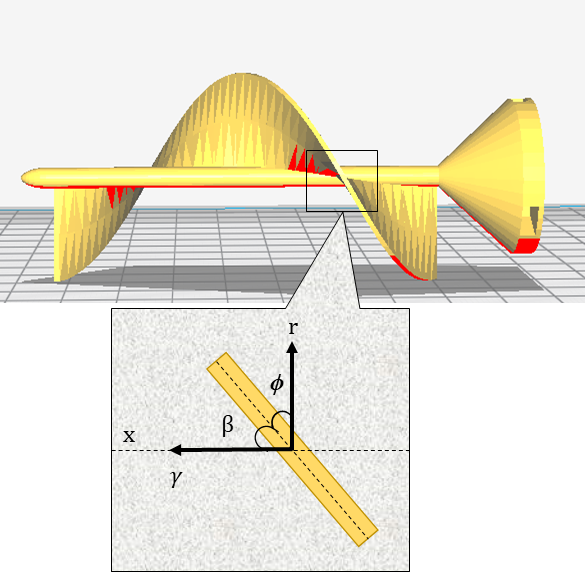
\includegraphics[height=9cm]{./imgs/helix_plate}
\caption{A plate element moving through granular media. Attack angle $\beta = \frac{\pi}{2} - \phi$ sets the tilt of the plate with respect to the horizontal plane. Intrusion angle $\gamma$ defines the direction the plate moves with respect to the horizontal plane. }
\label{fig:helix_plate}
\end{figure}

With explicit equations known for $F_x(\phi,U)$, $C_t$, and $C_n$, an aggressive auger was designed by first setting $R = \SI{0.02}{\m}$ and $n = 1$. These values were arbitrarily chosen since $R$ and $n$ do not influence $U$ when drag and thrust are balanced. Algorithm 1, using equations (\ref{FxAuger}, \ref{chenCt}-\ref{chenCn}), was then implemented to predict $U$ for different values of $\phi$ [Figure \ref{fig:UvPhi}]. Shown below, the maximum value of $U$ (\SI[per-mode=fraction]{8.19736e-2}{\m\per\s}) occurs when $\phi = \phi_{opt} = \SI{23}{\degree}$.   
\begin{figure}[H]
\centering
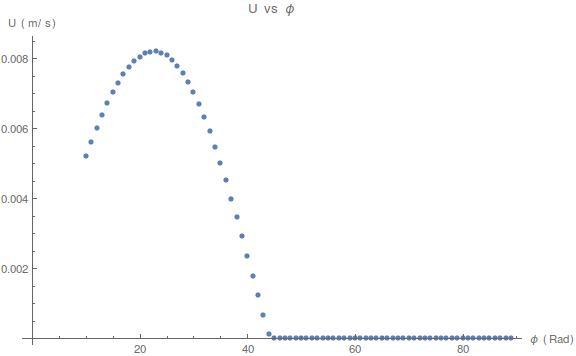
\includegraphics[width=0.7\linewidth]{./imgs/UvPhi}
\caption{$U$ (\si{\m/\s}) vs. $\phi$ (\si{\radian}) for a prone auger ($R$ = \SI{0.02}{\m}, $n = 1$, and $\omega = $ \SI[per-mode=fraction]{3.51}{\radian\per\s}) moving in the x-direction buried at a depth of $d =$ \SI{0.05}{\m} in loosly packed poppy seeds. $\phi$ was varied from \SI{10}{\degree} to \SI{90}{\degree} in increments of \SI{1}{\degree}.}
\label{fig:UvPhi}
\end{figure}
 
\section{Optimized Augerbot Observations and Future Directions}
In SolidWorks, a new auger was modeled with dimensions corresponding to the optimal parameters found using algorithm 1 [Table \ref{optParamTable}]. Compared to the helices tested previously [Figure \ref{fig:all_screws}], the thickness of the profile swept along the path of the screw was increased to ensure the threads merged properly with the stem.   

\begin{table}[H] 
\begin{center}
\caption{Optimized Auger and Test Bed Parameters}
	\begin{tabular}{ l l}
	\textbf{Parameter} & \textbf{Value} \\
	Radius (R) & \SI{0.02}{\m} \\
	Revolutions (n) & 1 \\
	Angular velocity ($\omega$) & \SI{3.51}{\radian\per\s} \\
	Depth (d) & \SI{0.05}{\m}\\  
	Local inclination ($\phi_{opt}$) & \SI{23}{\degree}\\
	Sweep thickness & \SI{0.0025}{\m}
	\end{tabular}
	\label{optParamTable}
\end{center}
\end{table}

\medskip
Figure \ref{fig:final_robot} shows the optimized auger prototype fastened onto the head of the robot. Like before, surface-skimming, diving and submerged experiments were run in a loosely packed bed of poppy seeds. The locomotive behaviors exhibited by the new robot were then compared against those observed for previous iterations. Wings parallel to the horizontal plane (\SI{0}{\degree}) and wings tiled \SI{30}{\degree} with respect to the horizontal plane were also mixed and matched to adjust the trajectory of the robot.  

\begin{figure}[H]
\centering
\begin{subfigure}{.5\textwidth}
	\centering
	\includegraphics[height=6cm]{./imgs/final_robot}
	\caption{The optimized burrowing robot}
	\label{fig:final_robot}
\end{subfigure}%
\begin{subfigure}{.5\textwidth}
	\centering
	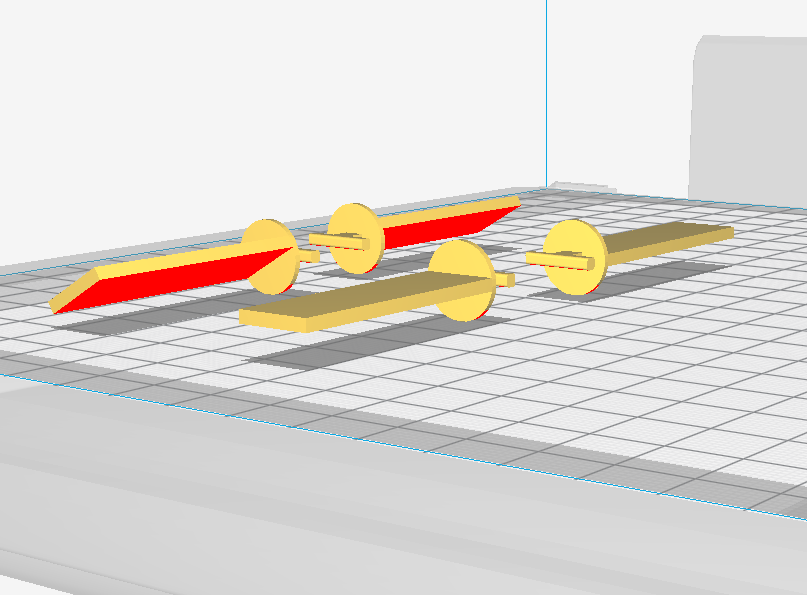
\includegraphics[height=6cm]{./imgs/wings}
	\caption{Wings angled at \SI{0}{\degree} and \SI{30}{\degree}}
	\label{fig:wings}
\end{subfigure}
\caption{Modular components used to tune the optimized robot}
\label{fig:final_testing}
\end{figure} 

When the robot is buried horizontally \SI{0.05}{\m} underground, it does not advance forward. Instead, the auger tilts out of the poppy seed bed within a span of 2 seconds. Looking at the geometry of the auger, it is evident that a stress gradient, in the direction of gravity, contributes to the upward bias of the robot's motion. To counter this tendency to surface, wings with a downward pitch could be added to ensure neutral buoyancy. Additional trim flaps could also be added continuously to actively control the dive angle of the auger's nose. 
 
When the robot is placed horizontally on the surface of a freshly fluidized (i.e level) poppy seed bed, it spirals in the clockwise direction due to the right-handed asymmetry of the auger - regardless of the wing configuration. This behavior matches that exhibited by previous prototypes. Larger wings or a rudder could be installed to counter the torque generated. A left-handed auger also be added adjacent to the existing right-handed auger. 
 
When the robot penetrates the poppy seed bed at a sufficiently shallow angle with respect to the horizontal plane, some axial translation is observed. Pointing the nose of the auger downwards prevents the robot from resurfacing immediately, giving it enough time to pull itself forward. This observation reinforces the need for larger, downward-pitched wings and the development of actuated wing flaps.   

\section{Conclusion}


\bibliographystyle{plain}
\bibliography{burrowing_biblio}

\end{document}